\documentclass[12pt,a4paper,oneside]{memoir}
\usepackage{polski}
\usepackage[top=2.5cm, bottom=2.5cm, left=3.5cm, right=1cm]{geometry}
\usepackage{amsmath}
\usepackage{amsfonts}
\usepackage{amssymb}
\usepackage{graphicx}
\usepackage{titling}
\usepackage{titlesec}
\usepackage{fontspec}
\usepackage{siunitx}
\usepackage{caption}
\usepackage{multirow}
\usepackage{lscape}
\usepackage[table,xcdraw]{xcolor}
\usepackage{float}
\usepackage[
bookmarks=false,
pdfpagelabels=false,
hyperfootnotes=false,
hyperindex=false,
pageanchor=false,
hidelinks
]{hyperref}
% Wykorzystywane źródła dla tego tekstu
% Usunięcie napisu "Rozdział"
\renewcommand{\chaptername}{} 
% Konwersja znaku mikro z matematyki na tekst
\sisetup{math-micro=\text{µ},text-micro=µ} 
% Ustawienie czcionki Arial 
\newfontfamily{\tytulyrozdzialow}{Arial} 
% Czionka TMR dla całego tekstu
\setmainfont{Times New Roman}
\titleformat
	{\chapter} % Formatowanie rozdziałów
	[hang] % Tekst obok liczby
	{\fontsize{14pt}{16pt}\bfseries\tytulyrozdzialow\flushleftright} % Regulacja czcionki rozdziałów
	{\chaptertitlename\ \thechapter.} % Ustawianie wyglądu nagłówków rozdziałów
	{15pt} % Odstęp między liczbą a tekstem
	{} 
\setsecheadstyle{\fontsize{13pt}{15pt}\tytulyrozdzialow\bfseries} % Ustawienie stylu dla sekcji
\begin{document}
\renewcommand{\maketitle}
{
	\centering
	
\includegraphics[scale=0.1]{images/logo.jpg}\par\vspace{1cm}
	{\scshape\LARGE Kierunek: Elektronika i Telekomunikacja\\ Specjalność: Teleinformatyka \par}
	\vspace{1cm}
	{\scshape\Large Praca dyplomowa inżynierska\par}
	\vspace{1.5cm}
	{\huge\bfseries Stacja meteorologiczna oparta o ESP8266\par}
	\vspace{2cm}
	{\Large\itshape Damian Zaręba\\Nr albumu 8389\par}
	\vfill
	Promotor:\par
	dr inż. Tadeusz Leszczyński
	\vfill
	
	% Dół strony
	{\large Mława 2019r. \par}
}
\maketitle
\thispagestyle{empty}
\newpage
{\tytulyrozdzialow \tableofcontents}
\newpage
\flushleftright
\chapter{Wstęp}
	\hspace{\parindent} Celem pracy jest zaprojektowanie i zrealizowanie stacji meteorologicznej opartej o mikroprocesor ESP8266, złożonej z kilku modułów. Aby zrealizować założony cel, zrealizowane zostały następujące zadania:
	\begin{itemize}{}{}
		\item Zaprojektowanie i wykonanie płyty głównej z mikrokontrolerem ESP8266EX dla przetwarzania informacji z sensorów oraz sterowania zasilaniem całego urządzenia;
		\item Zaprojektowanie i wykonanie anemometru do pomiaru kierunku i prędkości wiatru ze względów na koszty, ponieważ gotowe są zbyt drogie w stosunku do reszty;
		\item Zaimplementowanie sensora firmy BOSCH o nazwie BME280, który służy do odczytu temperatury, ciśnienia i wilgotności powietrza;
		\item Zaimplementowanie czujnika firmy PLANTOWER o nazwie PMS7003, który mierzy ilość pyłu zawieszonego w powietrzu, o wielkości PM1.0, PM2.5 oraz PM10, mierzone w \si\micro g/m$^{3}$.
	\end{itemize}
	\par W kolejnych rozdziałach pracy przedstawiono schemat blokowy urządzenia oraz ogólny opis poszczególnych modułów wykorzystanych do zbudowania tego urządzenia, wliczając w to charakterystyki głównych komponentów dla każdego modułu. Udokumentowane zostało m.in. konfiguracja środowiska, które zostało wykorzystana do stworzenia tego projektu.
	\par Przeanalizowano szczegółowo schemat urządzenia, a konkretnie płyty głównej, sekcji zasilania dla wykorzystanych sensorów oraz innych elementów niezbędnych do realizacji projektu. Poddana dokładnej analizie będzie każda z części schematu, takie jak sekcja zasilania czy połączeniowa między płytą główną a sensorami.
	\par Przedstawiono i opisano algorytmy oraz kod źródłowy programu sterującego stacją pogodową oraz omówiono protokoły komunikacyjne. Wykonuje on wiele zadań, m.in. odczytuje dane z sensorów czy kontroluje układy zasilania poszczególnych części.
	\par W przedostatnim rozdziale przedstawiono krótko projekt anemometru służącego do pomiaru prędkości i kierunku wiatru. Omówiony i opisany został schemat blokowy anemometru i jego elektryczna reprezentacja.
	\par W ostatnim rozdziale przedstawione zostały wyniki badań wykonanego modelu stacji pogodowej.

\chapter{Elementy składowe projektu} 
\section{ESP8266EX}
\par ESP8266EX to mikroukład z pełnym stosem TCP/IP oraz mikrokontrolerem wyprodukowanym przez Espressif w Szanghaju, Chiny.\\
Istnieje jego odmiana o nazwie ESP8285 z 1 MiB wbudowanej pamięci typu flash, co umożliwiało wykorzystanie go jako pojedynczego układu zdolnego do podłączenia się do sieci Wi-Fi, po podłączeniu zasilania. W odróżnieniu od rodziny mikrokontrolerów AVR nie może być zasilany napięciem 5V, jedynie 3.3 wolta.\\
\begin{figure}[h]
	\centering
	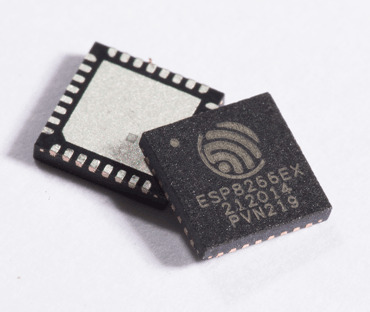
\includegraphics[scale=0.5]{images/esp8266ex.jpg}
	{\tytulyrozdzialow \footnotesize \caption[ESP8266EX]{Zdjęcie przedstawiające układ ESP8266EX}
	\caption*{\textit{Źródło: \cite{esp8266chip}}}}
\end{figure}\\
\par ESP8266EX \cite{esp8266wiki} posiada 32 bitowy procesor oparty o rdzeń Xtensa Diamond Standard 106Micro (LX106) firmy Tensillica o nominalnej wartości zegara wynoszącym 80 MHz. Charakteryzuje się on następującymi funkcjami:
\begin{itemize}
	\item 16 pinów GPIO
	\item SPI
	\item I$^2$C (programowa implementacja)
	\item I$^2$S z funkcją Direct Memory Access (współdzieli piny z GPIO)
	\item UART na wyznaczonych pinach GPIO oraz dodatkowy UART na GPIO2 służący jedynie do wysyłania danych
	\item 10-bitowy ADC oparty o sukcesywną aproksymację.
	\item Wbudowana obsługa Wi-Fi o standardach b/g/n według IEEE 802.11 z wbudowanym przełącznikiem TR,LNA,Balunem, wzmacniaczem mocy oraz siecią dopasowującą oraz możliwością podłączenia się lub tworzenia sieci z zabezpieczeniami WEP lub WPA/WPA2
\end{itemize}
\par Pamięć ulotna tego mikrokontrolera jest podzielona w następujący sposób :
\begin{itemize}
	\item 32 KiB RAM dla instrukcji
	\item 32 KiB RAM typu cache dla instrukcji
	\item 80 KiB RAM dla danych użytkownika
	\item 16 KiB RAM typu ETS dla danych "systemowych"
\end{itemize}
\par Obsługuje pamięć nieulotną typu flash po protokole SPI do pojemności 16 MiB, choć zazwyczaj korzysta się z pamięci o rozmiarach 512 KiB lub 4 MiB.\\
\begin{figure}[h]
	\centering
	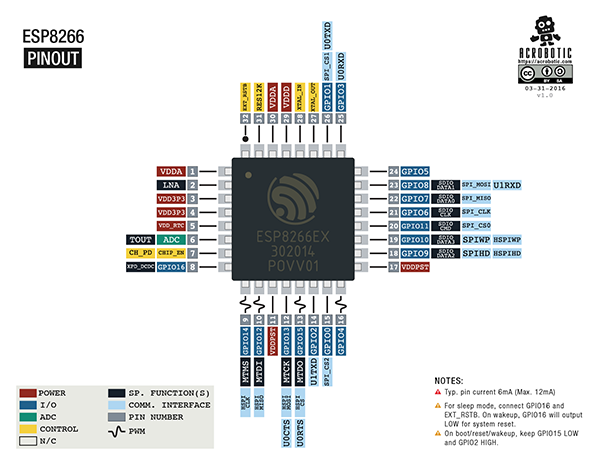
\includegraphics[scale=1.5]{images/esp8266_pinout.png}
	{\tytulyrozdzialow \footnotesize \caption[ESP8266EX - opis wyprowadzeń]{Zdjęcie przedstawiające wyprowadzenia dla układu ESP8266EX}
	\caption*{\textit{Źródło: \cite{esp8266pinout}}}}
\end{figure}
\newpage
Układ ESP8266EX posiada kilka linii zasliania:
\begin{itemize}
	\item 2x VDDA (Zasilanie sekcji analogowej)- 2.5 wolt do 3.6 wolt
	\item VDDD (To samo, co VDDA) - 2.5 wolt do 3.6 wolt.
	\item 2x VDD3P3 (Zasilanie wzmacniacza sygnału Wi-Fi) - 2.5 wolt do 3.6 wolt.
	\item 2x VDDPST (Zasilanie sekcji cyfrowej i wejść/wyjść) - 1.8 wolt do 3.6 wolt.
\end{itemize}
\par Używa się pinów GPIO2, GPIO0 oraz GPIO15/MTDO dla ustawienia trybu uruchamiania układu.
\\[10pt]
\begin{table}[!h]
\centering
\resizebox{10cm}{!}{%
	\begin{tabular}{|
			>{\columncolor[HTML]{EFEFEF}}c |c|c|c|}
		\hline
		\cellcolor[HTML]{96FFFB} & \cellcolor[HTML]{EFEFEF}\textbf{GPIO0} & \cellcolor[HTML]{EFEFEF}\textbf{GPIO2} & \cellcolor[HTML]{EFEFEF}\textbf{GPIO15} \\ \hline
		\textbf{\begin{tabular}[c]{@{}c@{}}Tryb \\ programowania\end{tabular}} & L & H & L \\ \hline
		\textbf{\begin{tabular}[c]{@{}c@{}}Uruchamianie z\\ pamięci flash\end{tabular}} & H & H & L \\ \hline
		\textbf{\begin{tabular}[c]{@{}c@{}}Uruchamianie z\\ karty SD\end{tabular}} & X & X & H \\ \hline
	\end{tabular}%
}
	{\tytulyrozdzialow \footnotesize \caption[ESP8266EX - tryby uruchamiania]{Tabela przedstawiająca tryby uruchamiania dla układu ESP8266EX}
	\caption*{\textit{Źródło: \cite{esp8266datasheet}}}}
\end{table}\\
\newpage
\par ESP8266EX obsługuje 14 kanałów w łączności Wi-Fi
\begin{table} [!h]
\centering
\resizebox{6cm}{!}{%
	\begin{tabular}{|c|c|}
		\hline
		\rowcolor[HTML]{EFEFEF} 
		\textbf{\begin{tabular}[c]{@{}c@{}}Numer\\ kanału\end{tabular}} & \textbf{\begin{tabular}[c]{@{}c@{}}Częstotliwość\\ {[}MHz{]}\end{tabular}} \\ \hline
		1 & 2412 \\ \hline
		2 & 2417 \\ \hline
		3 & 2422 \\ \hline
		4 & 2427 \\ \hline
		5 & 2432 \\ \hline
		6 & 2437 \\ \hline
		7 & 2442 \\ \hline
		8 & 2447 \\ \hline
		9 & 2452 \\ \hline
		10 & 2457 \\ \hline
		11 & 2462 \\ \hline
		12 & 2467 \\ \hline
		13 & 2472 \\ \hline
		14 & 2484 \\ \hline
	\end{tabular}%
}
	{\tytulyrozdzialow \footnotesize \caption[ESP8266EX - kanały Wi-Fi]{Tabela przedstawiająca dostępne kanały łączności Wi-Fi dla układu ESP8266EX}
	\caption*{\textit{Źródło: \cite{esp8266datasheet}}}}
\end{table}\\
\newpage
\par Maksymalny pobór prądu przez sam układ, nie licząc łączności Wi-Fi wynosi 12mA.
Pobór wzrasta w zależności od mocy transmisji lub odbioru pakietów za pomocą Wi-Fi. Pomiary były wykonane dla napięcia 3 wolt w temperaturze 25$^°$C. Wszystkie pomiary przesyłu danych były bazowane na 50\% długości cyklu
\begin{table}[!h]
\centering
\resizebox{15cm}{!}{%
	\begin{tabular}{|
			>{\columncolor[HTML]{EFEFEF}}c |c|c|c|c|}
		\hline
		\textbf{\begin{tabular}[c]{@{}c@{}}Parametry \\ łączności\end{tabular}} & \cellcolor[HTML]{EFEFEF}\textbf{Minimalny} & \cellcolor[HTML]{EFEFEF}\textbf{Typowy} & \cellcolor[HTML]{EFEFEF}\textbf{Maksymalny} & \cellcolor[HTML]{EFEFEF}\textbf{Jednostka} \\ \hline
		\begin{tabular}[c]{@{}c@{}}TX 802.11b\\ CCK 11 Mbps\\ $P_{OUT}$ =\\ +15 dBm\end{tabular} & - & 170 & - & mA \\ \hline
		\begin{tabular}[c]{@{}c@{}}TX 802.11g\\ OFDM 54 Mbps\\ $P_{OUT}$=\\ +17 dBm\end{tabular} & - & 140 & - & mA \\ \hline
		\begin{tabular}[c]{@{}c@{}}TX 802.11n\\ MCS7\\ $P_{OUT}$ =\\ +13 dBm\end{tabular} & - & 120 & - & mA \\ \hline
		\begin{tabular}[c]{@{}c@{}}RX 802.11b\\ 1024 bajtów\\ -80 dBm\end{tabular} & - & 50 & - & mA \\ \hline
		\begin{tabular}[c]{@{}c@{}}RX 802.11g\\ 1024 bajtów\\ -70 dBm\end{tabular} & - & 56 & - & mA \\ \hline
		\begin{tabular}[c]{@{}c@{}}RX 802.11n\\ 1024 bajtów\\ -65 dBm\end{tabular} & - & 56 & - & mA \\ \hline
	\end{tabular}%
}
	{\tytulyrozdzialow \footnotesize \caption[ESP8266EX - pobór mocy przy łączności Wi-Fi]{Tabela przedstawiająca pobór mocy dla łączności Wi-Fi przez ESP8266EX}
	\caption*{\textit{Źródło: \cite{esp8266datasheet}}}}
\end{table}
\newpage
\section{BME280}
BME280 to sensor temperatury, wilgotności i ciśnienia wykonany przez firmę Bosch.
Jego rozmiary to 2.5 milimetra na 2.5 milimetra w obudowie typu LGA (Land Grid Array).
Komunikuje się z mikrokontrolerem za pomocą protokołu I$^2$C (Do 3.4 MHz) lub SPI (3 lub 4 przewodowego, do 10 MHz)
\begin{figure} [h]
	\centering
	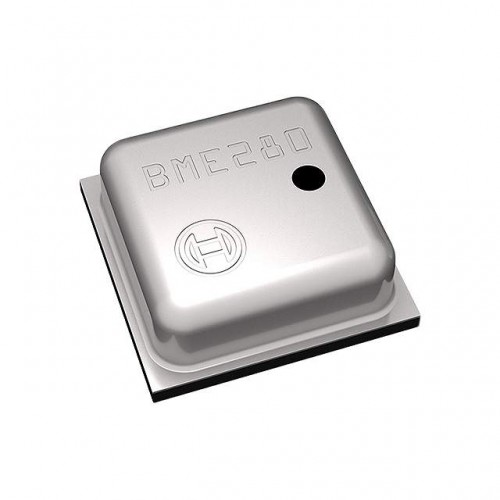
\includegraphics[scale=0.4]{images/bme280.jpg}
	{\tytulyrozdzialow \footnotesize \caption[BME280]{Zdjęcie przedstawiające układ BME280}}
	\caption*{\textit{Źródło: \cite{bme280chip}}}
\end{figure}\\
Zasilany jest w projekcie napięciem 3.3V, choć jego specyfikacja podaje, że pin zasilania VDD samego układu toleruje napięcia od 1.71 wolt do 3.6 wolt, a pin zasilania wejść/wyjść VDDIO od 1.2 wolt do 3.6 wolt.\\*
\begin{figure} [h]
	\centering
	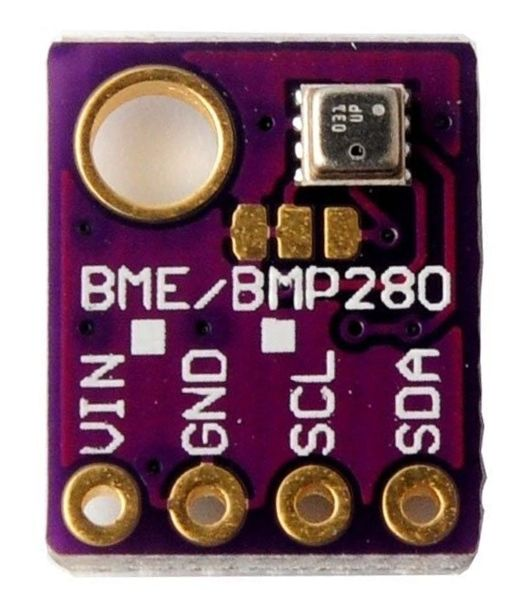
\includegraphics[scale=0.25]{images/bme280-mod.jpg}
	{\tytulyrozdzialow \footnotesize \caption[BME280 - Moduł]{Zdjęcie przedstawiające moduł zawierający BME280, komunikujący się przez protokół I$^2$C}}
	\caption*{\textit{Źródło: \cite{bme280module}}}
\end{figure}\\
\newpage
Pobiera w zastosowanej aplikacji około 3.6µA, czyli pomiaru wilgotności, ciśnienia i temperatury z częstotliwością 1Hz, choć może być niższy, ponieważ pomiary będą dokonywane rzadziej, około co pół godziny lub godzinę, w zależności od wymagań. Będzie możliwość ustawienia tego w kodzie źródłowym programu dla tej aplikacji.\\[10pt]
Kluczowe parametry sensora wilgotności:
\begin{itemize}
	\item Czas odpowiedzi ($\tau_{63\%}$) wynosi 1 sekundę
	\item Tolerancja dla dokładności pomiaru wynosi ±3 \% relatywnej wilgotności
	\item Histereza pomiaru wynosi ±1 \% relatywnej wilgotności
\end{itemize}
Kluczowe parametry części pomiarowej dla ciśnienia:
\begin{itemize}
	\item Średni poziom szumów wynosi 0.2 Pa, co jest odpowiednkiem dla 1.7 cm
	\item Współczynnik odchylenia temperaturowego wynosi ±1.5 Pa/K, co jest równoważne dla ±12.6 cm przy zmianie temperatury o 1$^°$C
\end{itemize}
\newpage
\section{PMS7003}
Sensor PMS7003 służy do pomiaru ilości cząsteczek w powietrzu o gradiacji PM1.0, PM2.5 oraz PM10 (odpowiednio: cząsteczki o średnicy około 1µm, 2.5µm oraz 10µm). Powszechnie korzyta się z niego do pomiaru jakości powietrza. Wykorzystuje on do tego laserowy czujnik pyłków.
\begin{figure}[h]
	\centering
	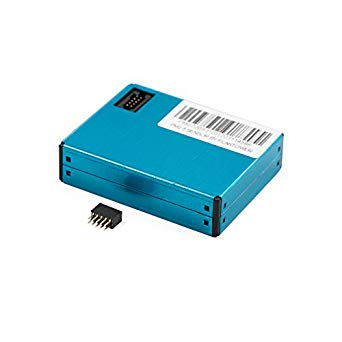
\includegraphics[scale=0.5]{images/pms7003.jpg}
	{\tytulyrozdzialow \footnotesize \caption[PMS7003] {Zdjęcie przedstawiające moduł PMS7003, komunikujący się przez protokół UART}}
	\caption*{\textit{Źródło: \cite{pms7003module}}}
\end{figure}\\
Czujnik ten charakteryzuje się następującymi parametrami:
\begin{itemize}
	\item Pojedynczy czas odpowiedzi wynosi mniej niż 1s
	\item Całkowity czas odpowiedzi wynosi do 10 sekund
	\item Zasilany jest napięciem 5 wolt
	\item Pobór prądu podczas pomiarów wynosi do 100 mA
	\item Stały pobór prądu, kiedy czujnik nie wykonuje pomiaru wynosi do 200 μA
	\item Napięcie operacyjne dla przesyłu i odbioru danych to 3.3 wolta.
	\item Pracuje w temperaturze od -10 do +60 stopni Celcjusza.
	\item "Pojemność" czujnika wynosi 0.1L
\end{itemize}
\begin{figure}[ht]
	\centering
	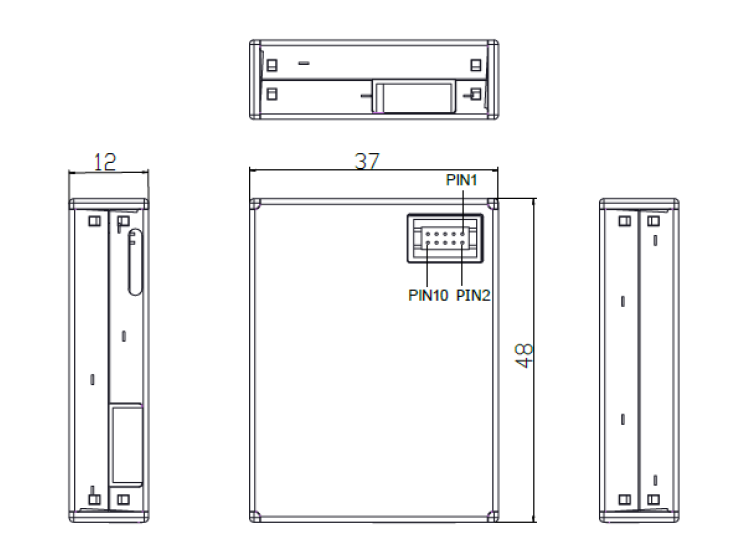
\includegraphics[scale=0.5]{images/pms7003-pinout.png}
	{\tytulyrozdzialow \footnotesize \caption[PMS7003 - pinout] {Zdjęcie przedstawiające wyprowadzenia czujnika PMS7003}
	\caption*{\textit{Źródło: \cite{pms7003datasheet}}}}
\end{figure}
\newpage
Lista wyprowadzeń tego sensora jest następująca:
\begin{table}[h]
	\centering
	\resizebox{10cm}{!}{%
	\begin{tabular}{|c|c|c|}
		\hline
		\multicolumn{3}{|c|}{\cellcolor[HTML]{EFEFEF}\textbf{Wyprowadzenia PMS7003}} \\ \hline
		Pin 1 & VCC & Zasilanie 5V \\ \hline
		Pin 2 & VCC & Zasilanie 5V \\ \hline
		Pin 3 & GND & Masa zasilania \\ \hline
		Pin 4 & GND & Masa zasilania \\ \hline
		Pin 5 & RESET & Pin resetu modułu \\ \hline
		Pin 6 & NC & - \\ \hline
		Pin 7 & RX & Pin odbierania danych \\ \hline
		Pin 8 & NC & - \\ \hline
		Pin 9 & TX & Pin wysyłania danych \\ \hline
		Pin 10 & SET & \begin{tabular}[c]{@{}c@{}}Stan wysoki - normalna operacja\\ Stan niski - uśpienie układu\end{tabular} \\ \hline
	\end{tabular}%
}
	{\tytulyrozdzialow \footnotesize \caption[PMS7003 - Lista wyprowadzeń] {Tabela przedstawiająca listę wyprowadzeń modułu PMS7003}}
	\caption*{\textit{Źródło: \cite{pms7003datasheet}}}
\end{table}
\newpage
\chapter{Wykorzystane protokoły komunikacyjne}
\section{I$^2$C}
\par I$^2$C \cite{i2cwiki} to protokół szeregowy zaprojektowany przez firmę Phillips Semiconductor, która dziś działa jako NXP Semiconductors w 1982 roku. Ma możliwość podpięcia wielu urządzeń w trybie \textit{Master} oraz w trybie \textit{Slave}. Istnieją dwie dodatkowe wersje I$^2$C - SMBus (System Management Bus), wykorzystywany w komputerach klasy PC do zarządzania podzespołami oraz PMBus (Power Management Bus) - do kontroli urządzeń związanych z zasilaniem. 
\par Wykorzystuje on dwie obustronne linie z otwartym kolektorem lub otwartym drenem, Serial Data Line (SDA) i Serial Clock Line (SCL), z rezystorami podiągającymi do zasilania.Zazwyczaj używa się napięć +5V lub +3.3V, ale inne napięcia są również dozwolone.
\par Magistrala I$^2$C posiada kilka trybów prędkości:
\begin{itemize}
	\item Low-speed - 10 kbit/s
	\item Standard - 100 kbit/s
	\item Fast - 400 kbit/s
	\item Fast mode plus (Fm+) - 1 Mbit/s
	\item High speed - 3.4 Mbit/s
\end{itemize}
\par Z tych najszybszych korzysta się w systemach wbudowanych a nie w komputerach osobistych.\\
\par Magistrala I$^2$C posiada dwie ważne cechy - rozszerzanie zegara (Clock Stretching) oraz Arbitraż (Arbitation). 
Rozszerzanie zegara polaga na tym, że urządzenie typu \textit{Slave} może utrzymywać linię zegara SCL w stanie niskim po otrzymaniu lub wysłaniu bajtu informacji, która wskazuje, że nie jest jeszcze gotowe do przetwarzania kolejnej porcji danych. Urządzenie typu \textit{Master} komunikujące się z danym modułem nie może wtedy zakończyć transmisji tylko musi czekać aż linia zegara SCL będzie w stanie wysokim. Jest to jedyna sytuacja, gdzie urządzenie typu \textit{Slave} ma kontrolę nad linią zegara. Urządzenie typu \textit{Master} musi odczekać dodatkowe 4 μs po prześciu linii SCL w stan wysoki zanim będzie mógł podciągnąć linię zegara do stanu niskiego.
\par Magistrala I$^2$C posiada deterministyczny system arbitrażu. Arbitraż polega na tym, że każde urządzenie typu \textit{Master} monitoruje linię, wyszukując bitów START i STOP i nie zacznie komunikacji, póki linie są zajęte przez inne urządzenia typu \textit{Master}. Jednakże, dwa urządzenia typu \textit{Master} mogą zacząć transmisję w tym samym czasie - wtedy następuje arbitraż. Każdy transmiter sprawdza poziom linii danych (SDA) i porównuje do oczekiwanego; jeśli się nie zgadza to urządzenie transmitujące traci arbitrację i wyłącza się z danej interakcji z protokołem I$^2$C.
\newpage
\begin{table}[!h]
	\centering
	\resizebox{\textwidth}{!}{%
		\begin{tabular}{cccccc}
			\multicolumn{6}{c}{Status zajętości magistrali oraz bitów START i STOP.} \\ \hline
			\rowcolor[HTML]{EFEFEF} 
			\multicolumn{1}{|c|}{\cellcolor[HTML]{EFEFEF}\textbf{Typ}} & \multicolumn{1}{c|}{\cellcolor[HTML]{EFEFEF}\textbf{\begin{tabular}[c]{@{}c@{}}Linia Nieaktywna \\ (N)\end{tabular}}} & \multicolumn{1}{c|}{\cellcolor[HTML]{EFEFEF}\textbf{\begin{tabular}[c]{@{}c@{}}Start \\ (S)\end{tabular}}} & \multicolumn{1}{c|}{\cellcolor[HTML]{EFEFEF}\textbf{\begin{tabular}[c]{@{}c@{}}Oczekiwanie\\ (I)\end{tabular}}} & \multicolumn{1}{c|}{\cellcolor[HTML]{EFEFEF}\textbf{\begin{tabular}[c]{@{}c@{}}Stop\\ (P)\end{tabular}}} & \multicolumn{1}{c|}{\cellcolor[HTML]{EFEFEF}\textbf{\begin{tabular}[c]{@{}c@{}}Rozszerzanie zegara\\ (CS)\end{tabular}}} \\ \hline
			\multicolumn{1}{|c|}{\cellcolor[HTML]{EFEFEF}\textbf{Opis}} & \multicolumn{1}{c|}{Arbitraż wolny do zajęcia} & \multicolumn{1}{c|}{\begin{tabular}[c]{@{}c@{}}Zajmowanie linii\\ (Master)\end{tabular}} & \multicolumn{1}{c|}{\begin{tabular}[c]{@{}c@{}}Linia zajęta\\ (Master)\end{tabular}} & \multicolumn{1}{c|}{\begin{tabular}[c]{@{}c@{}}Zwalnianie linii\\ (Master)\end{tabular}} & \multicolumn{1}{c|}{\begin{tabular}[c]{@{}c@{}}Zastopowanie\\ (Slave)\end{tabular}} \\ \hline
			\multicolumn{1}{|c|}{\cellcolor[HTML]{EFEFEF}\textbf{SDA}} & \multicolumn{1}{c|}{Podciąganie pasywne} & \multicolumn{1}{c|}{\textbf{\begin{tabular}[c]{@{}c@{}}Zbocze opadające\\ (Master)\end{tabular}}} & \multicolumn{1}{c|}{\textbf{\begin{tabular}[c]{@{}c@{}}Stan niski\\ (Master)\end{tabular}}} & \multicolumn{1}{c|}{\textbf{\begin{tabular}[c]{@{}c@{}}Zbocze wzrastające\\ (Master)\end{tabular}}} & \multicolumn{1}{c|}{\begin{tabular}[c]{@{}c@{}}Nie ma \\ znaczenia\end{tabular}} \\ \hline
			\multicolumn{1}{|c|}{\cellcolor[HTML]{EFEFEF}\textbf{SCL}} & \multicolumn{1}{c|}{Podciąganie pasywne} & \multicolumn{1}{c|}{Podciąganie pasywne} & \multicolumn{1}{c|}{Pasywne podciąganie} & \multicolumn{1}{c|}{Pasywne podciąganie} & \multicolumn{1}{c|}{\textbf{\begin{tabular}[c]{@{}c@{}}Stan niski\\ (Slave)\end{tabular}}} \\ \hline
		\end{tabular}%
	}
	{\tytulyrozdzialow \footnotesize \caption[I$^2$C - Stany zajętości magistrali] {Tabela przedstawiająca stany zajętości linii w magistrali I$^2$C}}
	\caption*{\textit{Źródło: \cite{i2cwiki}}}
\end{table}
\begin{table}[!h]
	\centering
	\resizebox{1.05\textwidth}{!}{%
\begin{tabular}{|c|c|c|c|c|c|c|}
	\hline
	\rowcolor[HTML]{EFEFEF} 
	\cellcolor[HTML]{EFEFEF} & \multicolumn{2}{c|}{\cellcolor[HTML]{EFEFEF}\textbf{\begin{tabular}[c]{@{}c@{}}Wysłanie jednego bitu danych (1) (0)\\ (Linia SDA jest ustawiona po SCL w celu uniknięcia wykrycia fałszywego stanu linii)\end{tabular}}} & \multicolumn{2}{c|}{\cellcolor[HTML]{EFEFEF}\textbf{\begin{tabular}[c]{@{}c@{}}Odpowiedź odbiorcy za pomocą bitu ACK\\ (Bajt odebrany od nadawcy)\end{tabular}}} & \multicolumn{2}{c|}{\cellcolor[HTML]{EFEFEF}\textbf{\begin{tabular}[c]{@{}c@{}}Odpowiedź odbiorcy za pomocą bitu NACK\\ (Bajt nie odebrany od nadawcy\end{tabular}}} \\ \cline{2-7} 
	\rowcolor[HTML]{EFEFEF} 
	\multirow{-2}{*}{\cellcolor[HTML]{EFEFEF}\textbf{Typ}} & \textbf{Ustawienie bitów (Bs)} & \textbf{Gotowość do próbkowania (Bx)} & \textbf{Ustawienie bitów (Bs)} & \textbf{ACK (A)} & \textbf{Ustawienie bitów (Bs)} & \textbf{NACK(A')} \\ \hline
	\cellcolor[HTML]{EFEFEF}\textbf{Opis} & Nadawca ustawia bit (Master/Slave) & Odbiora próbkuje bit (Master/Slave) & \begin{tabular}[c]{@{}c@{}}Nadawca ustawia stan\\ wysokiej impedancji\end{tabular} & \begin{tabular}[c]{@{}c@{}}Nadawca widzi linię SDA\\ jako w stanie niskim\end{tabular} & \begin{tabular}[c]{@{}c@{}}Nadawca ustawia stan\\ wysokiej impedancji\end{tabular} & \begin{tabular}[c]{@{}c@{}}Nadawca widzi \\ stan wysoki\end{tabular} \\ \hline
	\cellcolor[HTML]{EFEFEF}\textbf{SDA} & Ustawia bit (Po opadnięciu SCL) & Odbiera bit (Po wzroście SCL) & \multicolumn{2}{c|}{\begin{tabular}[c]{@{}c@{}}Utrzymane w stanie niskim \\ (Po opadnięciu SCL)\end{tabular}} & \multicolumn{2}{c|}{\begin{tabular}[c]{@{}c@{}}Sterowane stanem wysokim \\ (Lub pasywnie wysokim) przez odbiorcę\\ (Po opadnięciu SCL)\end{tabular}} \\ \hline
	\cellcolor[HTML]{EFEFEF}\textbf{SCL} & \textbf{Opadające zbocze (Master)} & \textbf{Wzrastające zbocze (Master)} & \textbf{Opadające zbocze (Master)} & \textbf{Wzrastające zbocze (Master)} & \textbf{Opadające zbocze (Master)} & \textbf{Wzrastające zbocze (Master)} \\ \hline
\end{tabular}%
}
	{\tytulyrozdzialow \footnotesize \caption[I$^2$C - Stany magistrali przy przesyle danych] {Tabela przedstawiająca stany linii w magistrali I$^2$C przy wymianie informacji między odbiorcą a nadawcą}}
	\caption*{\textit{Źródło: \cite{i2cwiki}}}
\end{table}
Magistrala I$^2$C posiada 7 bitową adresację oraz 10 bitową adresację, która jest wykorzystywana jako rozszerzenie podstawowej, 7 bitowej adresacji. 7 bitowa adresacja posiada 2 zarezerwowane grupy adresów - \textit{0000 XXX} oraz \textit{1111 XXX}:
\begin{itemize}
	\item \textit{0000 000 0} - Generalne odwołanie
	\item \textit{0000 000 1} - bajt START
	\item \textit{0000 001 X} - Adres CBUS
	\item \textit{0000 010 X} - Zarezerwowane dla innego formatu magistrali
	\item \textit{0000 011 X} - Zarezerwowane na przyszły użytek
	\item \textit{0000 1XX X} - Kod trybu High Speed
	\item \textit{1111 1XX 1} - Kod identyfikacyjny urządzenia
	\item \textit{1111 0XX X} - 10 bitowa adresacja urządzenia typu \textit{Slave}
\end{itemize}
7-bitowa adresacja składa się z 7 bitów identyfikacji oraz ósmego bitu - oznaczenia zapisu/odczytu danych. Długość części MSB to 4 bity, a LSB - 3 bity.
\begin{table}[!h]
	\centering
	\resizebox{\textwidth}{!}{%
		\begin{tabular}{|c|c|c|c|c|c|c|c|c|c|c|c|c|}
			\hline
			\cellcolor[HTML]{EFEFEF}\textbf{Pole} & \cellcolor[HTML]{EFEFEF}\textbf{S} & \multicolumn{7}{c|}{Adres I$^2$C} & R/W & A & Sekwencje danych I$^2$C & P \\ \hline
			\rowcolor[HTML]{EFEFEF} 
			\textbf{Typ} & \cellcolor[HTML]{EFEFEF} & \multicolumn{8}{c|}{\cellcolor[HTML]{EFEFEF}\textbf{Pierwszy bajt}} & \cellcolor[HTML]{EFEFEF} & \cellcolor[HTML]{EFEFEF} & \cellcolor[HTML]{EFEFEF} \\ \cline{1-1} \cline{3-10}
			\rowcolor[HTML]{EFEFEF} 
			\textbf{Pozycja bitu w bajcie X} & \cellcolor[HTML]{EFEFEF} & \textbf{7} & \textbf{6} & \textbf{5} & \textbf{4} & \textbf{3} & \textbf{2} & \textbf{1} & \textbf{0} & \cellcolor[HTML]{EFEFEF} & \cellcolor[HTML]{EFEFEF} & \cellcolor[HTML]{EFEFEF} \\ \cline{1-1} \cline{3-10}
			\rowcolor[HTML]{EFEFEF} 
			\textbf{Pozycja 7-bitowego adresu} & \cellcolor[HTML]{EFEFEF} & \textbf{7} & \textbf{6} & \textbf{5} & \textbf{4} & \textbf{3} & \textbf{2} & \textbf{1} & \textbf{} & \cellcolor[HTML]{EFEFEF} & \cellcolor[HTML]{EFEFEF} & \cellcolor[HTML]{EFEFEF} \\ \cline{1-1} \cline{3-10}
			Opis & \multirow{-4}{*}{\cellcolor[HTML]{EFEFEF}\textbf{START}} & \multicolumn{4}{c|}{MSB} & \multicolumn{3}{c|}{LSB} & \begin{tabular}[c]{@{}c@{}}0 = Zapis\\ 1 = Odczyt\end{tabular} & \multirow{-4}{*}{\cellcolor[HTML]{EFEFEF}\textbf{ACK}} & \multirow{-4}{*}{\cellcolor[HTML]{EFEFEF}\textbf{\begin{tabular}[c]{@{}c@{}}Kolejny bajt itd.\\ Dalsze wiadomości zapisu\\ lub odczytu idą tutaj.\end{tabular}}} & \multirow{-4}{*}{\cellcolor[HTML]{EFEFEF}\textbf{STOP}} \\ \hline
		\end{tabular}%
	}
	{\tytulyrozdzialow \footnotesize \caption[I$^2$C - Struktura 7-bitowego adresu] {Tabela przedstawiająca strukturę 7-bitowej adresacji w magistrali I$^2$C}}
	\caption*{\textit{Źródło: \cite{i2cwiki}}}
\end{table}
\newpage
10-bitowy adres jest podzielony na 2 segmenty - górny i dolny, które są poprzedzone specjalnym adresem, który komunikuje, że wykorzystywana jest 10-bitowa adresacja w magistrali - \textit{1111 0XX X}.
\begin{figure}[!h]
	\centering
	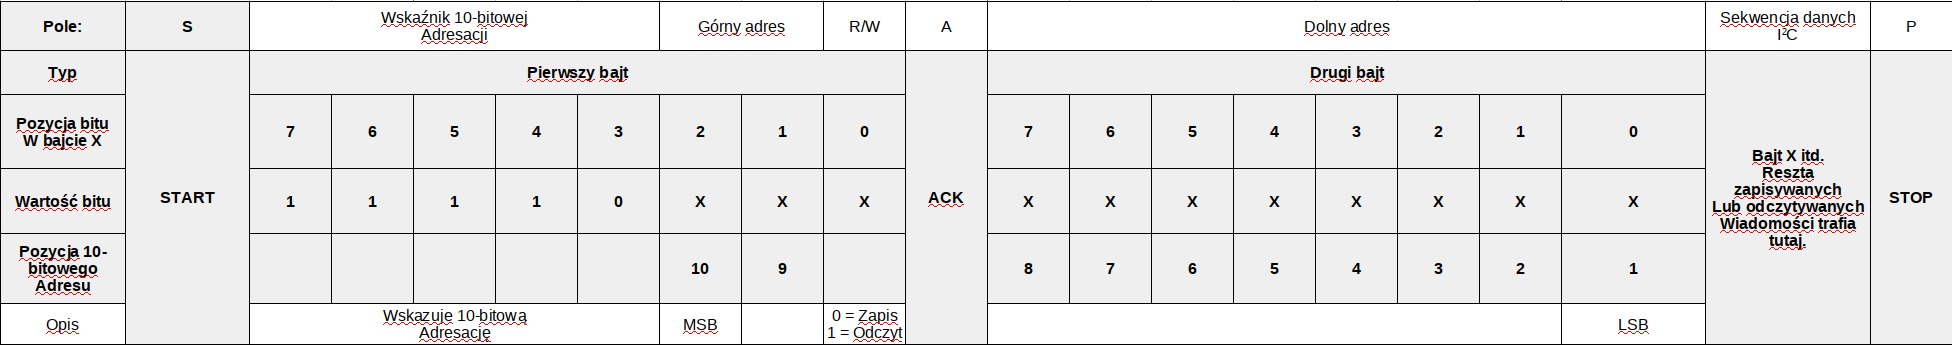
\includegraphics[scale=0.25]{images/i2c-10bit-addresing.png}
	{\tytulyrozdzialow \footnotesize \caption[I$^2$C - Struktura 10-bitowego adresu] {Tabela przedstawiająca strukturę 10-bitowej adresacji w magistrali I$^2$C}}
	\caption*{\textit{Źródło: \cite{i2cwiki}}}
\end{figure}\\
\newpage
Przebieg czasowy protokołu I$^2$C wygląda następująco:
\begin{enumerate}
\item Przesył danych jest inicjowany za pomocą bitu START (S) zasygnalizowane przez podciągnięcie linii SDA w stan niski, kiedy linia SCL jest w stanie wysokim;
\item Linia SCL jest podciągnięta do stanu niskiego, a linia SDA ustawia poziomu pierwszych bitów danych utrzymując linię SCL w stanie niskim (cała długość niebieskiego prostokąta);
\item Dane są próbkowane (odbierane) kiedy linia SCL jest w stanie wzrastającego zbocza dla pierwszego bitu. Żeby bit był poprawny, SDA nie może zmienić swojego stanu między wzrastającym zboczem linii SCL oraz następującym opadem zbocza (cała długość zielonego prostokąta);
\item Powyższa czynność jest powtarzana dla każdego kolejnego bitu;
\item Ostatni bit jest poprzedzony pulsem zegarowym, podczas którego linia SDA jest podciągnięta do stanu niskiego do przygotowania się do bitu STOP;
\item Bit STOP (P) jest sygnałowany kiedy linia SCL wzrasta, poprzedzona wzrastaniem linii SDA.
\end{enumerate}
\begin{figure}[!h]
	\centering
	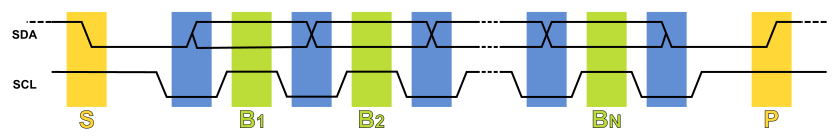
\includegraphics[scale=0.6]{images/i2c-timing.png}
	{\tytulyrozdzialow \footnotesize \caption[I$^2$C - Diagram czasowy] {Obrazek przedstawiający diagram czasowy w magistrali I$^2$C}}
	\caption*{\textit{Źródło: \cite{i2cwiki}}}
\end{figure}
\newpage
\section{UART}
\par UART (Universal asynchronous receiver-transmitter) \cite{uartwiki} to asynchroniczna, szeregowa magistrala komunikacyjna, w której format danych oraz prędkość przesyłu informacji jest konfigurowalna. Poziomy logiczne sygnałów oraz metody są kontrolowane przez zewnętrzną elektronikę podłączoną do kontrolera UART. Podobny protokół, USART (Universal synchronous and asynchronous receiver-transmitter) wspiera komunikację synchroniczną.
\par UART bierze bajty danych i przesyła indywidualne bity sekwencyjnie. W miejscu docelowym, urządzenie odbiorcze UART "buduje" dane na nowo z przybyłych bitów informacji w całe bajty. Każdy układ UART zawiera rejestr przesuwny, który odpowiada za przetwarzanie informacji między równoległą  a szeregową formą danych. Komunikacja może odbywać się w jednym z 3 trybów:
\begin{itemize}
	\item \textit{Simplex} - Tylko w jedną stronę, bez nadzoru dla urządzenia odbiorczego do wysyłu danych zwrotnych do urządzenia transmitującego;
	\item \textit{Half duplex} - Urządzenia zmieniają się miejscami przy przesyle danych - raz jedno wysyła, raz drugie;
	\item \textit{Full duplex} - Urządzenia wysyłają i odbierają dane w tym samym czasie.
\end{itemize}
\par W stanie oczekiwania, kiedy nie są wysyłane dane, linie są w stanie logicznym wysokim. Jest to pozostałość historyczna z telegrafów, gdzie linia była utrzymywana w stanie wysokim, żeby pokazać, iż linia i transmiter nie były uszkodzone.Każda część informacji jest opakowana jako bit START (logiczne 0), bity danych, opcjonalnie bit parzystości oraz jeden lub kilka bitów STOP.
\begin{figure}[!h]
	\centering
	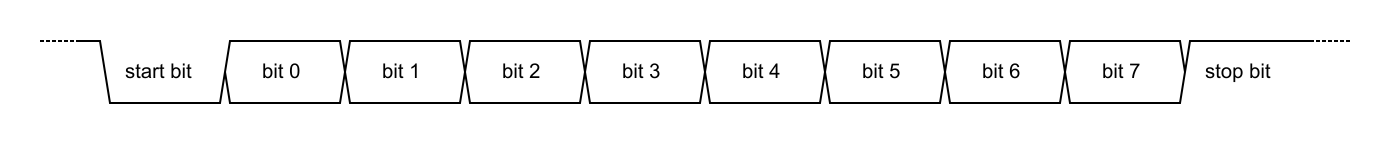
\includegraphics[scale=0.45]{images/uart-timing-diagram.png}
	{\tytulyrozdzialow \footnotesize \caption[UART - Diagram czasowy] {Obrazek przedstawiający diagram czasowy w magistrali UART}}
	\caption*{\textit{Źródło: \cite{uartwiki}}}
\end{figure}
\par Bit START sygnalizuje urządzenie odbiorcze o tym, że nowa częśc informacji nadchodzi. Kolejne 5 do 9 bitów, w zależności od odu który przyjęto, reprezentuje tą część danych. Jeśli bit parzystości został użyty, będzie umieszczony po wszystkich bitach danych. Kolejne 1 lub 2 bity zawsze są w oznaczonej pozycji (Logiczna jedynka) i nazwane bitem (lub bitami) STOP. Informują one moduł odbiorczy o tym, że ciąg znaków został ukończony.
\par UART składa się z kilku kluczowych elementów oraz ewentualnych, opcjonalnych dodatków, które rozszerzają możliwości magistrali w różny sposób.
Urządzenie  do obsługi protokołu UART wymaga:
\begin{itemize}
	\item Generator sygnału zegara, zazwyczaj wielokrotność prędkośći przesyłu danych dla umożliwienia próbkowania w środku czasu trwania bitu;
	\item Wejśćiowe i wyjśćiowe rejestry przesuwne;
	\item Kontrola przesyłu/odbioru danych;
	\item Logika kontrolijąca zapis/odczyt danych.
\end{itemize}
Dodatkowo, można wyposażyć protokół w dodatkowe bloki funkcyjne, takie jak:
\begin{itemize}
	\item Bufory przesyłu/odbioru danych;
	\item Bufor magistrali danych systemowych;
	\item Bufor pamięci typu FIFO (First-in, first-out);
	\item Sygnały potrzebne dla zewnętrznego kontrolera DMA (Direct Memory Access);
	\item Zintegrowana magistrala zarządzająca kontrolerem DMA.
\end{itemize}
\par UART posiada kilka specjalnych zdarzeń, które mogą wystąpić podczas transmisji. Są to:
\begin{itemize}
	\item Błąd przekroczenia (Overrun error) -Odbiornik nie może przetworzyć znaku który przybył przed kolejnym znakiem, który nadchodzi;
	\item Błąd niedociągnięcia (Underrun error) - Nadajnik skończył wysyłać dane i bufor przesyłu jest pusty;
	\item Błąd obramowania (Framing error) - Urządzenie nie "widzi" bitu STOP w oczekiwanym czasie jego występowania;
	\item Błąd parzystości (Parity error) - Bit parzystości nie zgadza się między odbiornikiem a nadajnikiem;
	\item Zerwanie transmisji (Break condition) - Wejście odbiornika jest w ,,odstępie" (Stan niski) dłużej niż przewidywany czas oczekiwania, zazwyczaj dłużej niż długość znaku.
\end{itemize}
\newpage
\chapter{Schemat funkcjonalny}
\par Zaprojektowane i wykonane urządzenie składa się z 3 głównych części - Dwóch różnych, wybieranych przez użytkownika źródeł zasilania (Zasilaczem lub baterią), sekcji zasilania mikrokontrolera i sensorów, oraz samego ESP8266EX i połączeń do wyprowadzeń dla czujników. Zasilanie jest czterokanałowe dla zapewnienia stabilności napięcia dla każdego ważnego układu w projekcie. Przełącznik pozwala na przełączanie między łądowaniem baterii a zasilaniem całej płyty głównej. Panel słoneczny jest bezpośrednio podłączony do kontrolera ładowania. 
\begin{figure}[!h]
	\centering
	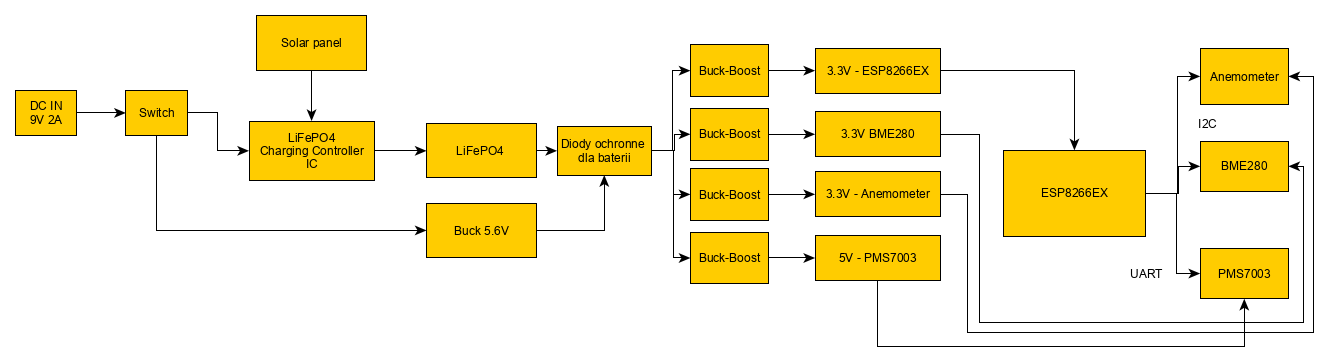
\includegraphics[scale=0.35]{images/block-schematic.png}
	{\tytulyrozdzialow \footnotesize \caption[Schemat blokowy] {Obrazek przedstawiający schemat blokowy urządzenia}}
	\caption*{\textit{Źródło: Opracowanie własne}}
\end{figure}
\par Wykorzystano baterię LiFePO4, które pozwalają na bardziej wydajną pracę od Li-Ion czy LiPo w temperaturach poniżej zera, ponieważ jedynie tracą około 10\% pojemności niżej zera stopni Celsjusza, nie 30+ \% jak Li-Ion czy LiPo. Wykorzystano przetwornice DC-DC typu buck-boost (push-pull) dla stabilizacji napięć z baterii LiFePO4. Mimo dużej ilości zakłóceń generowanych przez przetwornice DC-DC, posiadają o wiele wyższą sprawność od liniowych kontrolerów napięć. Dioda Schottky między baterią a przetwornicami uniemożliwi ładowania baterii napięciem 5.6V z kontrolera DC-DC który służy do zasilania całego układu przy odpowiednim ustawieniu przełącznika w tryb zasilania.
\newpage
\chapter{Schemat elektryczny}

\newpage
\chapter{Kod źródłowy} 

\newpage
\chapter{Opis anemometru} 

\newpage
\chapter{Infografika} 

\newpage
\listoffigures
\newpage
\listoftables
\newpage
\begin{thebibliography}{12}
	\bibitem{esp8266wiki}
	,,ESP8266'',
	\textit{Wikipedia},
	Zebrane 3 marca 2019,
	\url{https://en.wikipedia.org/wiki/ESP8266}
	\bibitem{esp8266datasheet}
	Nota katalogowa ESP8266,
	\textit{Espressif},
	Zebrane 25 lutego 2019,
	\url{https://www.espressif.com/sites/default/files/documentation/0a-esp8266ex_datasheet_en.pdf}
	\bibitem{esp8266chip}
	Zdjęcie ESP8266EX,
	\textit{alphamicrowireless.com}
	Zebrane 3 marca 2019,
	\url{http://www.alphamicrowireless.com/media/562039/esp8266ex_370px.gif}
	\bibitem{esp8266pinout}
	Pinout ESP8266EX,
	\textit{acrobotic.com},
	Zebrane 3 marca 2019,
	\url{https://learn.acrobotic.com/uploads/esp8266_pinout.png}
	\bibitem{bme280datasheet}
	Nota katalogowa BME280,
	\textit{Bosch},
	Zebrane 25 lutego 2019,
	\url{https://ae-bst.resource.bosch.com/media/_tech/media/datasheets/BST-BME280-DS002.pdf}
	\bibitem{bme280chip}
	Zdjęcie przedstawiające układ BME280,
	\textit{dnatechindia.com}
	Zebrane 3 marca 2019,
	\url{http://www.dnatechindia.com/image/cache/catalog/bme280\%201-500x500.jpg}
	\bibitem{bme280module}
	Zdjęcie przedstawiające gotowy moduł z układem BME280,
	\textit{gunook.com}
	Zebrane 3 marca 2019,
	\url{http://img.gunook.com/upload/a/1d/a1d0568812635b491d33f680db52a587.jpg}
	\bibitem{pms7003datasheet}
	Przetłumaczona nota katalogowa PMS7003,
	\textit{github.com}
	Zebrane 26 lutego 2019,
	\url{https://raw.githubusercontent.com/eleparts/PMS7003/master/data\%20sheet/PMS7003\%20datasheet.pdf}
	\bibitem{pms7003module}
	Zdjęcie sensora PMS7003,
	\textit{amazon.com}
	Zebrane 3 marca 2019,
	\url{https://images-na.ssl-images-amazon.com/images/I/41KI\%2BnbtAGL._SX342_.jpg}
	\bibitem{i2cwiki}
	,,I$^2$C'',
	\textit{Wikipedia}
	Zebrane 3 marca 2019,
	\url{https://en.wikipedia.org/wiki/I%C2%B2C}
	\bibitem{uartwiki}
	,,Universal asynchronous receiver-transmitter'', 
	\textit{Wikipedia}
	Zebrane 3 marca 2019,
	\url{https://en.wikipedia.org/wiki/Universal_asynchronous_receiver-transmitter}	
\end{thebibliography}

\newpage
\chapter{Streszczenie} 

\end{document}